\chapter{Choosing an architecture}
\label{sec:ChoosingArchitecture}

This chapter will view what goes into choosing a software architecture. What should you consider when choosing one and why.

A software architecture is:

\largequote{The process of converting software characteristics such as flexibility, scalability, feasibility, reusability, and security into a structured solution that meets the technical and the business expectations. \cite{softwareArchitectureDefinition}}

\section{Priorities}
\label{sec:Priorities}

As mentioned in the definition of software architecture, \fullref{sec:ChoosingArchitecture}, a software architecture looks at the characteristics as flexibility, scalability, ect. These characteristics and their sub characteristics are defined by ISO 25010 \cite{iso25010}. This is the standard that will be used troughout the research.

It is important to state the order in which EFFE values these quality attributes. Every decision will be based and rationalized by this order.

As mentioned in \fullref{sec:Intention} the first point points out the modularity and the interchangeability of these building blocks. The \textbf{maintainability} quality attribute has reusability and modularity as its sub characteristic. Thus is this the first focus of the software architecture.

Replaceability is a subcharacteristic of \textbf{portability}. As mentioned in \fullref{sec:TheProblem} the building blocks are interchangeable which goes hand in hand with replaceability.

The third focus is \textbf{compatability}. Compatibility is the degree in which a product, system or component can exchange information with other products, systems or components, and/or perform its required functions, while sharing the same hardware or software environment \cite{iso25010}. This is directly linked with the modularity of the system.

As mentioned in first and second point in \fullref{sec:Intention} the functionality may be shared between building blocks. But each building block should be able to function without other building blocks. This is why \textbf{functional sustainability} will be the fourth focus.

With such a loosely coupled system \textbf{security} becomes a bigger risk. Because every functionality is loosely coupled it means that the functionalities may talk with each other over a network instead of code. If it is an open network the security needs to be checked constantly. On a closed network measures need to be taken to keep the network closed. That is the reason why security is the fifth focus.

After running through these five quality attributes there is an application that can function without being overtaken by unintentional users. But in order to keep the intentional users satisfied the services or functions need to be reliable. Thus \textbf{reliability} will be the sixth focus.

If something is reliable it does not mean that it is usable. If the application is not responding as fast as possible there is a chance that the user will leave the application. A study conducted in 2018 by Google showed that there is a 58\% bounce rate when the load time is between 3 to 5 seconds \cite{bounceRateDifference}. Thus in order for the users to actually be able to use the application in a responsive manner \textbf{performance efficiency} becomes the seventh focus.

Normally there can be a solid argument made about why usability would be higher in the rankings. But because this research is more focussed on the architecture of the application and not UX or UI, \textbf{usability} is the eighth focus.

\subsection{Recap}
\label{sec:IsoRecap}

\begin{enumerate}
        \item Maintainability
        \item Portability
        \item Compatibility
        \item Functional sustainability
        \item Security
        \item Reliability
        \item Performance efficiency
        \item Usability
\end{enumerate}

\section{Creating an architecture}

Compared to choosing an architecture, creating one is something entirely different. An architecture does not exactly have a creator. An architecture is just blueprint on how to write the software. This is why the choice was made to interview software architects and ask them questions how they make their choices.

Before conducting the interview there is a need to have more information in order to frame the questions the right way. An architecture is assembly of implementations of certain features. These features are implemented to make the architecture fulfill a certain quality attribute. But each implementation has their drawbacks. These drawbacks can affect other quality attributes. This thought process is visualized in the figure \ref{fig:ChooseSoftwareArchitecture}.

The interviews showed that the understanding of software architecture portrayed in this research is the same as that of software architects. When explaining the thought process behind the image there was a positive feedback from the architects where they agreed that this is how they implement their own architectures and how they evaluate their implementations. The critique figure \ref{fig:ChooseSoftwareArchitecture} got, from one of the interviewees, is that maybe the software architect does not give priority to the quality attributes but the client of the product or the product owner does. This is because these parties formulate the requirements. This is reflected in figure \ref{fig:ChooseSoftwareArchitectureWReq}.

\begin{figure}[H]
	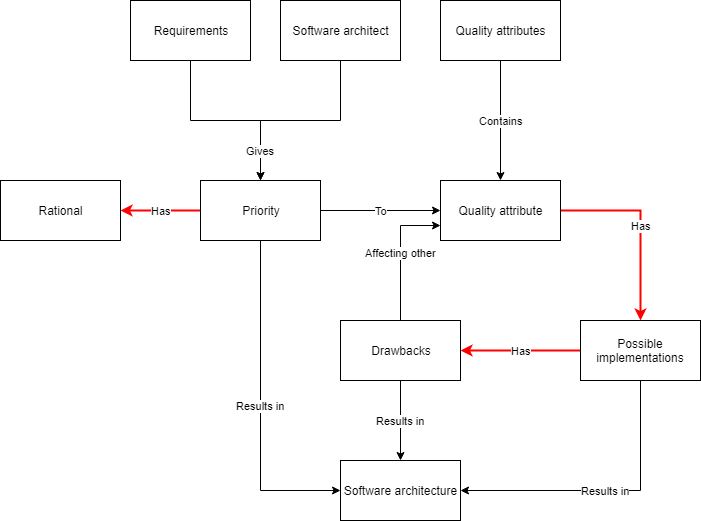
\includegraphics[width=\linewidth]{creating_architecture_requirements.png}
	\caption{How a software architecture is chosen with requirements}
        \label{fig:ChooseSoftwareArchitectureWReq}
\end{figure}
